%# -*- coding: utf-8 -*-
% !TEX encoding = UTF-8 Unicode
\RequirePackage{fixltx2e}
\documentclass[aps,pre,12pt,preprint,onecolumn,showpacs,showkeys,UTF8]{revtex4-1}
\usepackage{ctex}
\usepackage{mathrsfs}
\usepackage{setspace,dcolumn}
\usepackage{subfigure}
\usepackage{graphicx,psfrag,epsfig}
\usepackage[font=small,format=plain,labelfont=bf,textfont=it,justification=raggedright,singlelinecheck=false]{caption}
\usepackage{amsmath,amsfonts,amssymb,amsthm,bm,upgreek}
\usepackage{geometry}
\usepackage[mathscr]{eucal}
\usepackage{titlesec}
\usepackage{tabularx}
\titleformat{\section}{\bf\fangsong\zihao{4}}{\thesection}{0.75em}{}
\geometry{top=2.54cm,bottom=2.54cm,left=3cm,right=3cm}
\renewcommand\appendixname{附录}
\renewcommand\abstractname{}%摘要
\renewcommand\tablename{表}
\renewcommand\figurename{图}
\makeatletter
\def\@keys@name{\songti\zihao{-4}{\bf 关键词:}}
\def\Received@name{\zihao{-5}{接收} }
\def\Revised@name{\zihao{-5}{修订} }
\def\Accepted@name{\zihao{-5}{采纳} }
\def\Published@name{\zihao{-4}{发表} }
\makeatother
\linespread{1.6}
\renewcommand{\labelenumi}{\alph{enumi}.}
\leftmargini=20mm

\begin{document}

\title{\bf\heiti\zihao{3}硅的霍尔系数及电阻率的测量\vspace{15mm}}
\author{\fangsong 乔颢\vspace{2mm}}
\affiliation{\songti\zihao{-4}北京大学物理学院2011级2班~~~~学号:1100011354 \vspace{2mm}}
\keywords{半导体,电阻率,霍尔系数,范德堡法,杂质浓度}
\email{1993422qsh@gmail.com; 18600200672}
\begin{abstract}
	\vspace{10mm}
	\begin{spacing}{1.5}
		\songti\zihao{-4}本实验使用范德堡法测量得到了在不同温度下硅样品的电导率以及霍尔系数。研究了对应样品的空穴迁移率,杂质浓度等。计算的道了该样品的杂质浓度为$N_A=4.16\times10^2cm^{-3}$。禁带宽度为1.21eV。

	\end{spacing}
\end{abstract}

\maketitle

\section{引言}
霍尔效应是有关材料中的载流子在电场和磁场的作用下产生的效应。霍尔在1879年研究电导体在磁场中受力性质的时候发现了这种效应。半导体霍尔效应一直推动着固体导电理论的发展,尤其对于半导体电子论的发展有着极其重要的作用。霍尔系数和电导率的测量是分析半导体纯度和杂质种类的一种有理手段,至今仍是半导体材料和器件研制工作中的一种基本测试方法。通过在温度不同条件下的联合测量,可以得到更多的半导体电学参数。利用这些可以分析研究半导体的导电特性和机理。

本实验通过在不同温度下对于硅的霍尔系数和电阻率的测量,了解半导体本征导电和杂质导电两种导电机构,以及晶格散射杂质散射两种散射机构,并由此测量得到载流子的类型,禁带宽度,净杂质浓度,载流子浓度等等基本参数。


\section{实验装置}
本实验采用的实验装置示意图如\ref{g:1},是使用范德堡法测量样品的各种参数属性。将样品竖直的插入容器中,并且使用一个可以转动的魔环来提供一个恒磁场。磁场的方向相对于样品可以转动,从而可以改变霍尔效应所产生的影响。同时样品附近还有一系列的加热和测温装置,用于保持恒定的温度。以及对于这套设备的控制和测量部分,现实最终的数据以及控制系统的温度等等。

\begin{figure}[h]
	\begin{center}
		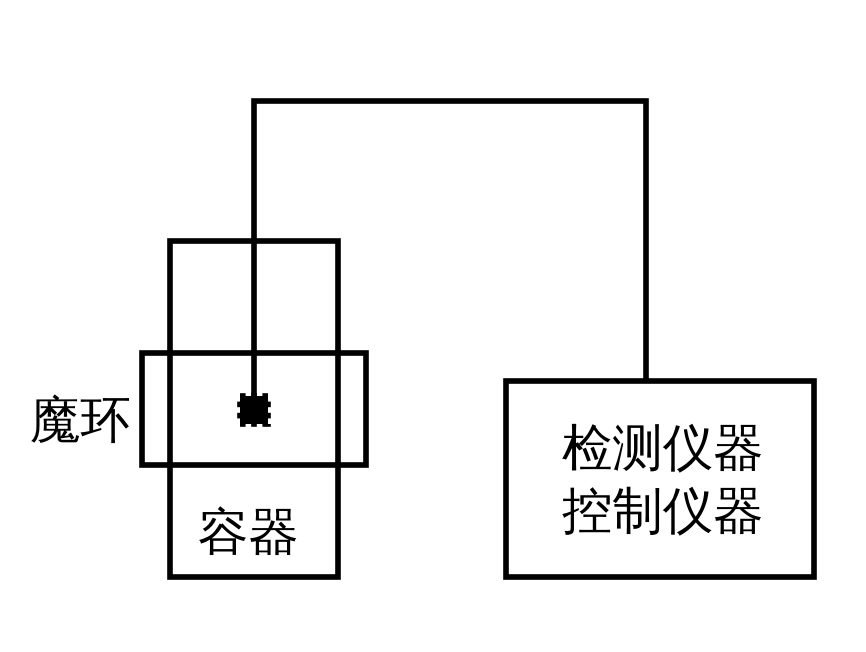
\includegraphics[width=0.7\textwidth]{pic1.png}
		\caption{\label{g:1}测量硅电阻率和霍尔系数的示意图。}
	\end{center}
\end{figure}

霍尔电压在垂直于磁场的方向产生,因此可以通过改变磁场的方向来引入或者移除测量端的霍尔效应,也能通过这个消除里纪-勒杜克效应。通过对于电阻率,霍尔系数的测量,更可以计算出这个半导体样品的具体参数,确定其详细的性质。具体的测量计算方法如下。
\section{实验步骤以及数据}
实验中需要测定的是样品的电阻率和霍尔系数随着温度变化的关系。所以采取以下方法测量。首先将温度恒定到一个稳定的温度并且使之保持稳定,调整磁场方向使得等效磁场为0(即磁场沿半导体平面方向)。这时候保持电流不变测量$V_I$$V_{II}$,以及反向之后的$V_I'$ $V_{II}'$后即可计算得到。同理可以通过测量$V_{III}$在有无磁场时电压的变化即可计算出来对应的霍尔系数。公式如下:
\begin{equation}
	\rho=\frac{\pi d}{\ln 2} \frac{V_I+V_{II}-V_I'-V_{II}'}{2i}f
\end{equation}
\begin{equation}
	R_H=\frac{d}{B}\frac{V_{III}(+I,+H)-V_{III}(+I,0)+V_{III}(-I,-H)-V_{III}(-I,0)}{2i}
\end{equation}

实验数据计算结果如下表\ref{t:1}所示:
\begin{center}
	\begin{table}[ht]
		\caption{测定得到硅的电导率和霍尔系数随温度的变化表,}
		\label{t:1}
		\begin{tabular}{m{3cm}<{\centering}m{3cm}<{\centering}m{3cm}<{\centering}m{3cm}<{\centering}}
			\hline
			\hline
			设定温度/$^{\circ}C$	&	样品温度/K	&	$\rho/\Omega\cdot cm^{-1}$	&	$R_H/10^4cm^3\cdot C^{-1}$	\\
\hline
室温	&	300.5	&	3252.42	&	88.03	\\
40	&	309.2	&	3440.06	&	83.95	\\
50	&	319.7	&	3596.65	&	77.50	\\
60	&	329.9	&	3653.54	&	69.47	\\
70	&	339.7	&	3618.64	&	60.00	\\
80	&	349.9	&	3482.44	&	48.16	\\
90	&	359.1	&	3256.84	&	33.68	\\
100	&	369.1	&	2874.42	&	15.53	\\
107	&	375.9	&	2489.63	&	3.42	\\
114	&	382.9	&	2015.54	&	-6.45	\\
121	&	389.7	&	1526.95	&	-11.58	\\
128	&	396.5	&	1086.63	&	-14.87	\\
135	&	403.9	&	743.19	&	-15.79	\\
141	&	410	&	568.70	&	-14.34	\\
144	&	412.7	&	511.93	&	-13.29	\\
147	&	415.6	&	452.67	&	-12.11	\\
150	&	418.3	&	408.48	&	-11.05	\\
153	&	421.1	&	363.72	&	-10.00	\\
156	&	424.2	&	322.02	&	-8.95	\\
159	&	427.3	&	285.43	&	-8.29	\\
162	&	430.4	&	253.70	&	-6.97	\\
166	&	434.6	&	215.40	&	-6.05	\\
\hline
\hline
		\end{tabular}
	\end{table}
\end{center}

做出$\ln \rho ~ (1000/T)$和$\ln |R_H| ~ (1000/T)$的曲线如下图\ref{g:2}所示,可以看出电导率在329.9K的时候达到了最大值,因此在温度小于此温度时为杂质电离饱和区。最高温度的时候空穴浓度远远大于杂质浓度,样品处于本征态的范围。
\begin{figure}[ht]
	\begin{center}
		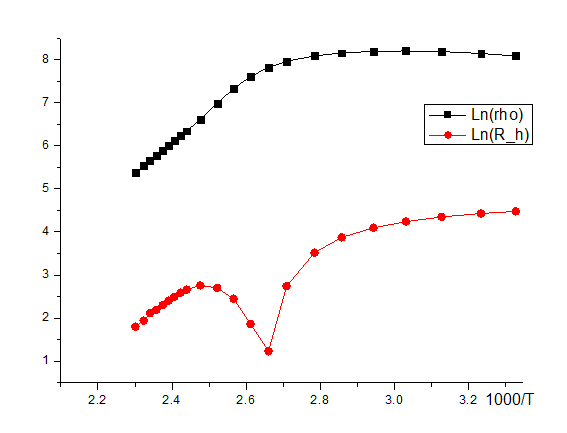
\includegraphics[width=0.6\textwidth]{pic2.png}
		\caption{\label{g:2}$\ln \rho$和$\ln |R_H|$与1000/T的关系图。}
	\end{center}
\end{figure}

取温度在杂质电离饱和区的四个数据,可以计算得到对应的空穴迁移率$\mu_{Lp}$。计算公式如下:
\begin{equation}
	(\mu_{Lp})_T=(\mu_{Lp})_{300}\frac{\sigma_T}{\sigma_{300}}
\end{equation}
做出的$\ln \mu_{Lp}-\ln T$的曲线如图\ref{g:3}所示,可以看出线性度不是十分的好,得到的数据关系为$\mu_{Lp}=(6\pm2)\times 10^5T^{-(1.2\pm0.2)}(cn^2/Vs)$,这个和Morin的公式有着很大的差距。这里可能是因为这更好的饱和范围并不是这四个点,而且数据点的个数太小,本身线性程度就不是特别的好,所以得到了差距很大的结果。
\begin{figure}[ht]
	\begin{center}
		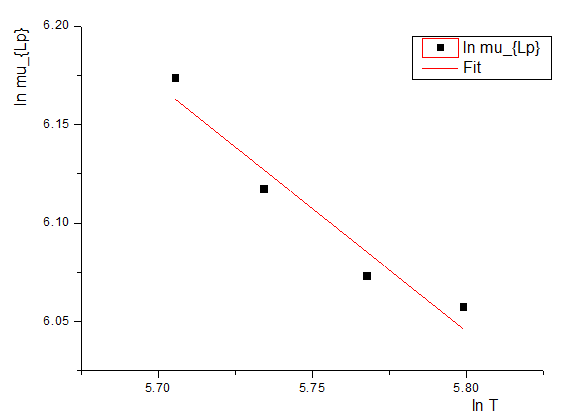
\includegraphics[width=0.6\textwidth]{pic3.png}
		\caption{\label{g:3}$\ln \mu_{Lp}$与ln T的关系图。}
	\end{center}
\end{figure}

根据$R_{Hmax}=-R_{Hs}\frac{(b-1)^2}{4b}$可以计算出b值为2.31。其中R的极值取为-15.69$\times10^4cm^3/C$。通过Morin共识计算得到的b的值为2.64。两者相对误差大约在12\%。这里误差来源可能是因为极值点并不精确,同时与饱和区的$R_H$的取值也有关系。

随后计算杂质浓度$N_A$。从$\ln\rho-(1000/T)$曲线得到300k的时候电阻率为3252.4$\Omega\cdot cm^{-1}$。从公式$N_A=\frac{1}{q\mu_{Lp}\rho}$可以计算得到对应的杂质浓度。有
\begin{equation}
	N_A=\frac{1}{q\mu_{Lp}\rho}=4.16\times10^2cm^{-3}
\end{equation}

在半导体处于本征激发的高温区时候,有空穴浓度和载流子浓度满足以下式子:
\begin{equation}
	p=(\frac{1}{q\mu_{Lp}\rho}+bp_s)/(b+1)
\end{equation}
\begin{equation}
	n=(\frac{1}{q\mu_{Lp}\rho)-p_s)/(b+1)}
\end{equation}
根据之前得到的$\ln \mu_{Lp}-\ln T$曲线可以得到对应温度的$\mu_{Lp}$。这样就可以计算得到p和n的值。并且可以做出$\ln p-(1000/T)$以及$\ln(\frac{p\cdot n}{T^3})-(1000/T)$的曲线,如图\ref{g:4}以及图\ref{g:5}所示。其中计算近禁带宽度的图中范围只取了本征激发的范围,这样情况下才能满足对应的公式。
\begin{figure}[ht]
	\begin{center}
		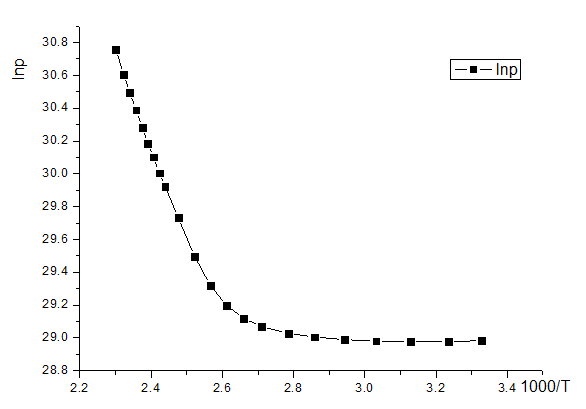
\includegraphics[width=0.6\textwidth]{pic4.png}
		\caption{\label{g:4}$\ln p$与(1000/T)的关系图,其中p为空穴浓度}
	\end{center}
\end{figure}
\begin{figure}[ht]
	\begin{center}
		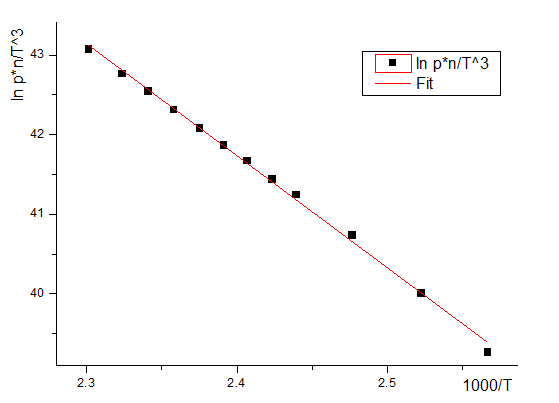
\includegraphics[width=0.6\textwidth]{pic5.png}
		\caption{\label{g:5}$\ln \frac{p\cdot n}{T^3}$与(1000/T)的本征激发时的关系图。其中n为空穴浓度}
	\end{center}
\end{figure}
可以看出$\ln \frac{p\cdot n}{T^3}$与(1000/T)的线性关系非常的好,可以计算出对应的禁带宽度$E_g=1.21eV$。
\section{结论}
本实验通过测量硅半导体样品的电导率以及霍尔系数,确定了样品在杂质电离饱和区的空穴迁移率为:
\begin{equation}
	\mu_{Lp}=(6\pm2)\times 10^5T^{-(1.2\pm0.2)}(cn^2/Vs)
\end{equation}
以及空穴载流子迁移率之比为2.31。杂质浓度为$N_A=4.16\times10^2cm^{-3}$。禁带宽度为1.21eV。
\section{致谢} 
感谢许福军老师的指导,以及贾春燕,冉书能老师的技术支持。

\begin{thebibliography}{}
	\bibitem{Book} 吴思成,王祖铨~2010 近代物理实验(第三版)(北京:高等教育出版社)第402页.%
%
\end{thebibliography}

\clearpage
\appendix
\section{思考题}
1、影响霍尔系数的正确测量的因素有很多,比如磁场的均匀性,测量温度与样品实际温度的差别,各种各样的副效应等等都会影响。可以使用更大的磁场范围更小的样品以增加均匀性质,使用更好的温度控制系统,等等都可以似的霍尔系数测量更精确。

2、优点是不容易发热,磁场比较稳定,没有对于稳定电源的要求等等。测量方法上电磁铁是采用交换电流方向改变磁场方向,而永磁魔环则是旋转方向即可。

3、温度控制器和温度计是两套测量系统,一个是铂电阻,一个是温差电偶。而且一个测量的是加热器附近的温度,另外一个则是测量的样品附近的温度,所以结果不一样很正常。调节电压时应该在低温是电压偏低,高温的时候增加功率。这样才能更好的达到稳定。

4、温度升高,半导体本征激发,从原来的杂质占主导变为了电子占主导,因而造成了霍尔电压的方向改变。
\end{document} 
